\subsection{Sensor Coordinate Transformations}
\label{subsec:transformations}

Each radar sensor in the dual-radar configuration is physically mounted with a specific orientation and tilt relative to the vehicle's forward direction. 
To ensure a common frame of reference for all points, it is necessary to compensate for:

\begin{itemize}
    \item \textbf{Yaw rotation}: due to angled placement (±30) of the radar modules.
    \item \textbf{Pitch tilt}: due to upward mounting tilt (+15), which must be compensated to recover horizontal geometry.
    \item \textbf{Sensor offset}: due to the physical separation of the radar sensors in the horizontal axis (X-axis).
\end{itemize}

We apply a yaw rotation \( R_{\text{yaw}} \), followed by a pitch correction \( R_{\text{pitch}} \), and finally apply a translation vector \( \vec{t} \) that accounts for the physical position of the sensor with respect to the vehicle's coordinate origin.

The full transformation can be expressed as:

\begin{equation}
T_{\text{veh}} = R_{\text{yaw}} \cdot R_{\text{pitch}} \cdot \vec{p}_{\text{radar}} + \vec{T}
\label{eq:radar_to_vehicle_transform}
\end{equation}

Where:
\begin{itemize}
    \item \( \vec{p}_{\text{radar}} \) is a radar point in sensor coordinates.
    \item \( R_{\text{yaw}} \) is a 2D or 3D rotation around the vertical axis.
    \item \( R_{\text{pitch}} \) corrects for the upward sensor tilt.
    \item \( \vec{T} \) is the translation vector
\end{itemize}

\vspace{1em}

Let $(x, y, z)$ be the original point from the radar frame, with $x$ to the right, $y$ forward, and $z$ upward. 
The transformations applied are as follows:

\paragraph{Yaw Correction (Z-axis Rotation)}
The radar sensors are rotated relative to the vehicle frame:

\begin{itemize}
    \item Radar A (Left): Mounted at $+30^\circ$ yaw $\Rightarrow$ Compensated with $-30^\circ$ rotation.
    \item Radar B (Right): Mounted at $-30^\circ$ yaw $\Rightarrow$ Compensated with $+30^\circ$ rotation.
\end{itemize}

The 2D rotation in the XY-plane is applied as:
\[
\begin{bmatrix}
x' \\
y'
\end{bmatrix}
=
\begin{bmatrix}
\cos(\theta) & -\sin(\theta) \\
\sin(\theta) & \cos(\theta)
\end{bmatrix}
\begin{bmatrix}
x \\
y
\end{bmatrix}
\]

where $\theta = \pm30^\circ$ depending on the sensor.

\begin{figure}[!htbp]
    \centering
    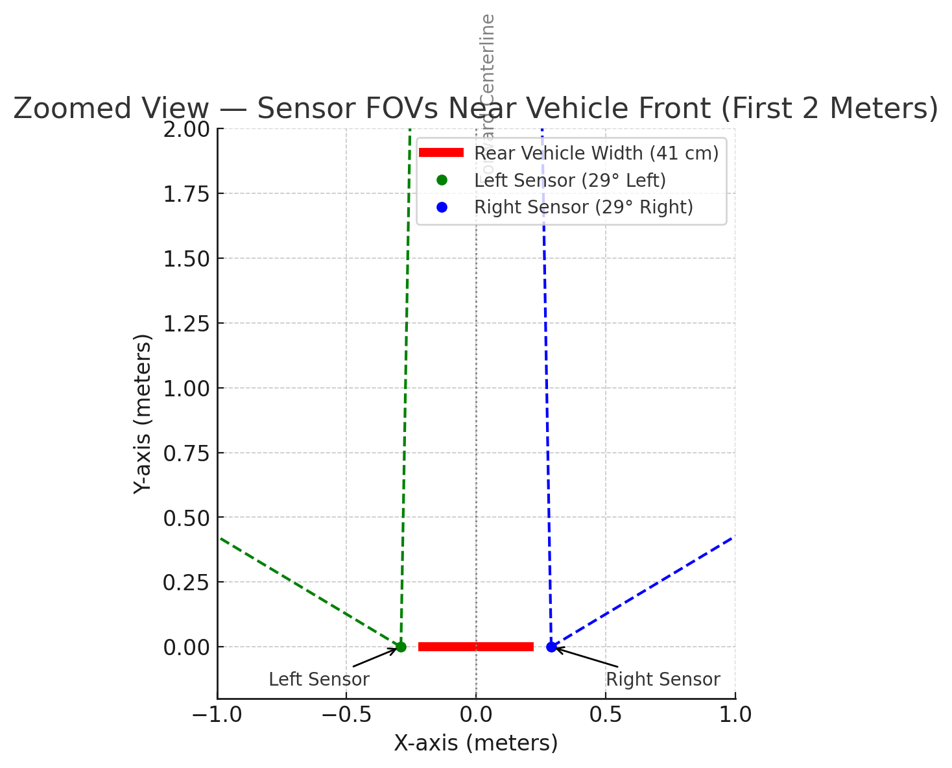
\includegraphics[width=1.0\linewidth]{images/SensorsRotation.png}
    \caption{Sensor rotation around Z axis.}
    \label{fig: Z axis rotation}
\end{figure}

\vspace{2em}

\paragraph{Pitch Compensation (X-axis Rotation)}
Due to the radar sensors being tilted upward by $15^\circ$, a corrective rotation around the X-axis is applied to bring the points back to a horizontal perspective. 
The transformation is:

\[
\begin{bmatrix}
x'' \\
y'' \\
z''
\end{bmatrix}
=
\begin{bmatrix}
1&0&0\\
0& \cos(\phi) & -\sin(\phi) \\
0& \sin(\phi) & \cos(\phi)
\end{bmatrix}
\begin{bmatrix}
x' \\
y' \\
z
\end{bmatrix}
\]

where $\phi = -15^\circ$ (negative to reverse the upward tilt).

\begin{figure}[!htbp]
    \centering
    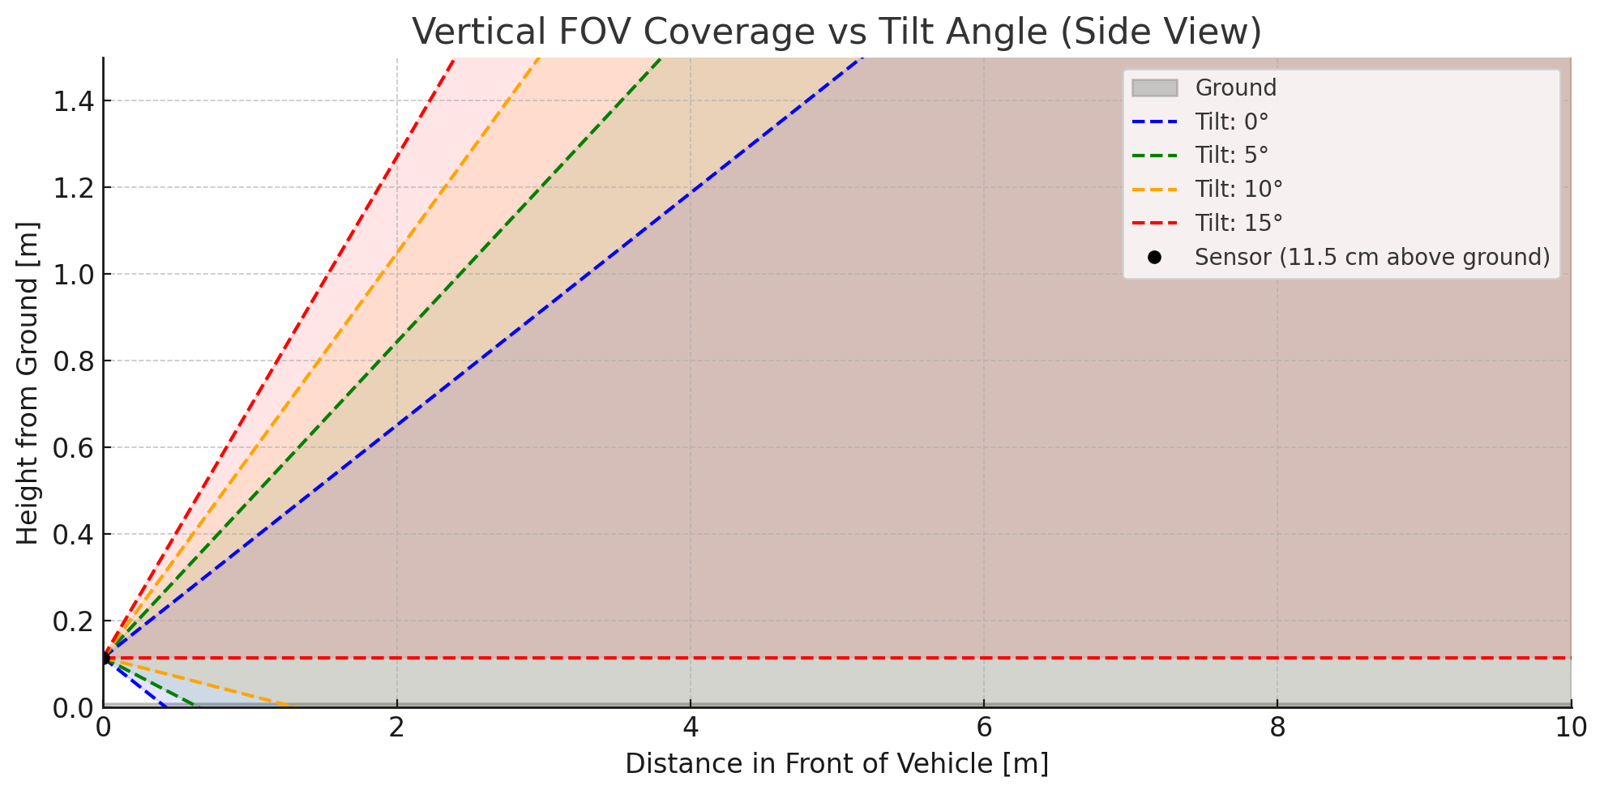
\includegraphics[width=1.0\linewidth]{images/TiltSensor.png}
    \caption{Sensor rotation around X axis.}
    \label{fig: X axis rotation}
\end{figure}

\paragraph{X-Axis Offset Compensation}
After rotation, each sensor's point cloud is translated along the X-axis to align with the vehicle's center:
\[
\mathbf{T}_{\text{A}} = 
\begin{bmatrix}
x \\
y \\
z
\end{bmatrix}
\]

\[
\mathbf{T}_{\text{B}} = 
\begin{bmatrix}
x \\
y \\
z
\end{bmatrix}
\]
\begin{itemize}
    \item Radar A: $x \leftarrow x - 0.32$ meters
    \item Radar B: $x \leftarrow x - 0.28$ meters
\end{itemize}

These transformations ensure that all point cloud data from both sensors are expressed in a unified vehicle-centric frame. 
This is essential for accurate point aggregation, ego-motion estimation, and object detection.
